%
The variety of \NIKA\ scientific targets going from thermal SZ observations to
dust polarization properties requires an accurate calibration process able
to define the impact of systematic errors on the final sky
maps as well as possible. The overall calibration uncertainty for point sources on the final data 
at the map level is estimated to be 
15~\% for the 1.25~mm channel and 10~\% for 2.14~mm channel.
In the following, a list of the principal error sources, which have a
direct impact on the total calibration uncertainties, is presented. In Table
\ref{tab:table_err}, we quantify these contributions.

\begin{figure*}[t!]
\begin{center}
\includegraphics[width=7cm]{figures/beam_profile_1mm.eps} 
\includegraphics[width=7cm]{figures/beam_profile_2mm.eps} \\
\includegraphics[width=7cm,trim=0cm 0.35cm 0cm 0cm,clip]{figures/Saturn_mapbeam_1mm.ps} 
\includegraphics[width=7cm,trim=0cm 0.35cm 0cm 0cm,clip]{figures/Saturn_mapbeam_2mm.ps} 
\end{center}
\caption{Top panel: Radial profile of the \NIKA\ beam pattern (red dots) including the secondary beam contribution for the 1.25~mm channel (left) and 2.14~mm channel (right) in the case of Uranus observations. We are able to measure the beam pattern profile up to scales of about 100 arcsec. At larger distances we do not have enough signal-to-noise. For illustration we also show the \NIKA\ measured primary beam. 
%The plots indicate that beyond a radius of 100 arcsec we do not have signal to noise
% enough to observe the fraction of the total beam contained at far larger distances. 
 Bottom panel: Map of the far side lobes for 1.25~mm channel (left) and for 2.14~mm channel (right). The maps are derived using observation of Saturn. These maps are compatible with the  the 2D structure of the beam pattern of the IRAM 30~m telescope described in \citep{Greve,kramer}). The diffraction ring seen at 1.25~mm at about 2~arcmin radius, corresponds to the diffraction ring  due to panel buckling. The spider supporting the secondary mirror of the telescope is visible to a level of about -30~dB.}
\label{fig:fsl}
   \end{figure*} 


\begin{itemize}

\item {\bfseries Primary calibrator}:  Uranus was selected as the primary calibrator 
for the \NIKA\ absolute calibration. The absolute calibration factor is derived by fitting 
a Gaussian of fixed angular size on the reconstructed maps of Uranus. 
The flux of Uranus is deduced from \cite{moreno2010,planckii}  using a frequency-dependent
model of the planet brightness temperature and integrating over the \NIKA\ bandpasses. We obtained brightness temperatures of 113~K at 2.14~mm and 94~K at 1.25~mm. This model is accurate at the 
level of 5~\%. 

\item {\bfseries Elevation dependent gain}: The IRAM 30~m telescope has 
a gain that changes with the elevation. This is because the antenna was not designed in a complete homology way. 
According to the design and measurements \citep{Greve, kramer}, the peak
of the elevation gain curve is obtained for an elevation of 43~degrees. 
Elevation gain variations have been corrected for in the data analysis.
%, and the
%rms increases up to approx. 55 $\mu m$ when moving in
%elevation to 0 or 90 degrees. This means that when the antenna goes 
%out of the optimum elevation, some part of the power
%goes out the antenna main beam. 

\item {\bfseries Spectral response}: The bandpasses as described in section
  \ref{instr} are obtained as an average of all pixels for each channel. This
  leads to a contribution to the total calibration error due to the dispersion
  of the measured bandpasses and to the slightly different response of the
  pixels.

\item {\bfseries FOV reconstruction}: To recover the
  pointing direction of each pixel, a focal plane reconstruction via planet
  scans is used. The accuracy of this technique has been described in Section~\ref{focal}.

\item {\bfseries Secondary beam fraction}: Planet observations were used to
  measure individual pixel primary beams as well as for the FOV
  reconstruction. The beam width is obtained by fitting a Gaussian on the
  planet maps. We have observed that variations in the atmospheric conditions
  lead to changes on the beam width. Since we calibrate assuming a fix beamwidth,
  these variations induce a systematic error in the final calibration.
  % which
  %is due to the secondary beams variation with atmospheric opacity.

\item {\bfseries Opacity correction}: The sky maps are
  corrected for the atmospheric contribution rescaling the observed signal by
  what that would be obtained in the absence of atmosphere. This
  is achieved via the elevation scan technique (skydip). The \NIKA\ skydip
  procedure was successfully tested during the last two \NIKA\ observing
  campaigns, and it produced a low-level dispersion of the derived opacity at
  different elevations.

\item {\bfseries Data reduction filtering}: 
The main steps in the data processing 
have been discussed in section \ref{dataprocessing}. The estimated systematic error 
introduced by the data reduction filtering (in particular due to the common modes subtraction) 
is estimated at 5~\% for both channels. This was computed from the dispersion between different
processing modes.

\end{itemize}

In the following we discuss the secondary beam fraction
contribution and the atmospheric absorption correction in more detail.

\subsection{Secondary beam fraction}
The secondary beam fraction needs to be estimated and accounted for in the case of extended sources. 
This is known by comparing the \NIKA\ beam pattern with the beam pattern of the 30~m telescope as measured by \cite{kramer} (K13) on the Lunar edge using the EMIR receiver. For practical purpose we have divided the beam into three regions: short angular scales correspond to the main beam, intermediate angular scales corresponding to the first error beam, and large angular scales assimilated to far side lobes of the 30m telescope. To compute the main beam we performed a Gaussian fit to the full observed NIKA beam pattern. The best Gaussian fit is shown in yellow. The \NIKA\ main beam is consistent with the one of K13 because we expect the main beam to be defined by the diameter of the 30~m telescope. In the same way far side lobes, which are expected to come mainly from the second and third error beams of the 30~m telescope caused by small adjustment errors of the panels and their frames, are also consistent between \NIKA\ and K13. However, the first error beam observed in the \NIKA\ beam pattern is larger than the one modeled by K13. This is not unexpected since the observations were carried out at a different time of day and under different weather conditions.
In Fig \ref{fig:fsl}, we show profiles and maps of the beam emphasizing the contribution of the secondary beam for both \NIKA\ channels. The results on the estimation of its contribution are presented in Table~\ref{tab:table_err}.

\subsection{Atmospheric absorption correction using a \Skydip\
  calibration}\label{skydips}

\begin{figure}
\begin{center}
\includegraphics[width=8cm]{figures/Fig_tel.eps} 
\includegraphics[width=9cm]{figures/skydip.eps}
\end{center}
\caption{Top: telescope positions during an elevation scan procedure: 10 steps in elevation have been performed without changing the azimuthal position. Data for absolute calibration are taken in the region
  between the blue and the red lines. Middle plot: signal in Hz of each valid
  KID (blue for 1.25~mm detectors, red for 2.14~mm) as a function of air mass, together with the fitted model (black dotted lines). Bottom plot: Histogram of the deduced
  integrated in-band opacities for the 1.25~mm and 2.14~mm channels.}
\label{fig:skydip}
\end{figure} 

%\textcolor{blue}{JFMP: I would not call this atmospheric calibration as we do not use the
%skydips to compute the calibration factor but rather the atmospheric
%absorption.} \\

In the previous observing campaigns, the atmospheric absorption correction
was made using the IRAM tau-meter that performs elevation scans continuously
at a fixed azimuth at 225~GHz. To derive the opacity at the exact position of
the scan and at the same frequencies as \NIKA\, we implemented a
procedure that uses the \NIKA\ instrument itself as a tau-meter. For the
last 2012 and 2013 observing campaigns, the \NIKA\ atmospheric calibration
consisted in measuring the variation in the resonance frequencies of the
detectors versus the airmass via elevation scans (\emph{skydip} \cite{dicke})
from 65 to 20 degrees above the horizon. The procedure is based 
on the idea that the KIDs response (the change in resonant frequency for a given 
change in absorbed power) is a constant property of each detector. This has been
demonstrated in laboratory under realistic conditions (with an optical load changing 
between about 50~K and 300~K, \cite{monfardiniLTD})

\begin{figure}[b!]
\begin{center}
\includegraphics[width=8cm]{figures/opa_run_all_notaumeter_v1.eps}
\end{center}
\caption{Atmospheric opacity evolution for the \NIKA\ 2012 and 2013 observing campaigns 
calculated from the \Skydip\ analysis. The error bars were estimated by
analysing different \Skydip\ observations. During the 2013 observing campaign, the agreement with 225~GHz IRAM taumeter is good.}
\label{fig:op}
\end{figure}

%The IRAM taumeter (225\,GHz) is shown for comparison (note that it showed some malfunctions during the 2012 campaign).

During \Skydip\, the telescope performs ten elevation steps each corresponding to variations of 0.18 in air
mass. We perform a tuning of the readout electronics before acquiring a useful signal. For
each step we have 22 seconds of useful signal at a given elevation. This is shown
in the top plot of  Figure~\ref{fig:skydip} where we present the observed elevation as a function
of time during the \Skydip\ procedure.

We expect the acquired useful signal per detector to respond to the airmass as:

\begin{equation}\label{eq:skydip}
F^{Ground}_{skydip} = F_0 + C T_{atm}[1 - e^{- x \tau_{skydip}}].
\end{equation}

Here, $F^{Ground}_{skydip}$ is the acquired signal corresponding to the
absolute value of the shift in the frequency tone for each pixel, $F_0$ is the
instrumental offset corresponding to the frequency tone excitation for the
considered pixel for zero opacity, $C$ the calibration conversion factor in
$\mathrm{Hz/K}$, $T_{atm}$ (in Kelvin) is the equivalent temperature of the
atmosphere, $\tau_{skydip}$ the sky opacity during the skydip (at the
wavelength of the fit, either 1.25 or 2.14~mm), $x$ the airmass 
with $x = sec(\delta)$  where $\delta$ is the average elevation
of the telescope during the scan. By performing a fit of the three
parameters, $F_0$, $C$, and $\tau$, for all valid detectors at the same
wavelengths, we obtain a common sky opacity at zenith during the skydip. We
can rerun the fit on each detector, assuming the common $\tau$ value, and get
the coefficients $F_0$ and $C$ per detector. In the middle and bottom panels of Fig.~\ref{fig:skydip} we
present the main results of the data analysis of one \Skydip\ performed during the
2013 campaign.

\begin{table*}
\begin{center}
\begin{tabular}{ccc}
\hline
\hline
Systematics & 1.25~mm Channel error &  2.14~mm Channel error  \\
\hline \hline
Secondary beams fraction$^*$  (cuts at $30^{"}$, $60{"}$, $90^{"}$) & 25\%, 41\%, 43\%   & 9\%, 30\%, 33\% \\
Primary calibrator &  5\% & 5\% \\
Elevation dependant gain correction$^{**}$ &  20\% & 10\% \\
Spectral response &  2\% & 1\% \\
FOV reconstruction & 3.4 arcsec & 3.2 arcsec \\
Opacity correction &  5\% & 6.5\%  \\
Data reduction filtering (on point sources)  &  5\% & 5\%  \\
\hline
\bfseries{Overall calibration}  & \bfseries{15\%} & \bfseries{10\%} \\
\hline \hline
\end{tabular}
\end{center}
\caption{Different contributions to the total calibration error of the \NIKA\ data. $^*$  is estimated by measuring the main beam volume ($2\pi \sigma^2$) over the integral of the beam volume up to a considered angular radius. $^{**}$ Typically for 1.25~mm the gain correction is about 8~\% at an elevation of 30~deg (3~\% at 2.14~mm).}
\label{tab:table_err}
\end{table*}

\begin{figure}[t!]
\begin{center}
\includegraphics[width=7cm]{figures/skydipvsATM_run5.ps} \\
\includegraphics[width=7cm]{figures/skydipvsATM_run6.ps}
\end{center}
\caption{Comparison between the atmospheric opacities measured with the \Skydip\ technique
  (blue points) and the ATM model (purple lines). The top plot is for the 2012
  campaign, the bottom plot for the 2013 campaign.}
\label{fig:skydipvsmodel}
\end{figure} 


%\begin{figure*}[t!]
%\begin{center}
%\includegraphics[width=7cm]{figures/integrated_beam_Run5_OTFUranus_1mm.ps} 
%\includegraphics[width=7cm]{figures/integrated_beam_Run5_OTFUranus_2mm.ps} 
%\end{center}
%  \caption{\textcolor{blue}{JFMP: Remi should add a caption here}}
%\label{fig:overall_error}
%   \end{figure*} 


The $F_0$, $C$ coefficients only depend on the response of the detectors.
Since the non-linearities of the KID frequency signal are negligible in the
considered range of backgrounds, the coefficients can be applied to all the
observing campaign to recover the opacity of the considered scan. This is
obtained by inverting Eq \ref{eq:skydip} as

\begin{equation}\label{eq:skydip2}
\tau_{scan_i}=\frac{1}{x_{scan}}\ln{(1-\frac{F^{Ground}_{scan_i}-F_{0_i}}{C_iT_{atm}})}.
\end{equation}
where $\tau_{scan_i}$ is the opacity of the considered scan as measured by a
given detector, $x_{scan}$ corresponds to the air mass at the elevation of the
considered scan, $F^{Ground}_{scan_i}$ is the measured absolute value of the
detector resonance frequency during the scan, and $F_{0_i}$ and $C_i$ are the
coefficients derived from the \Skydip\ technique. The opacity $\tau_{scan}$ is
deduced by averaging $\tau_{scan_i}$ for all valid detectors at a given
wavelength. The brightness of the observed scan map $S^{Ground}$ can be
rescaled onto the scale that would be obtained using detectors outside the
atmosphere ($S^{Star}$) with

\begin{equation}
S^{Star} =  S^{Ground} \cdot e^{ x \tau_{scan}}.
\end{equation}

A initial advantage of this method is that we do not need to perform the \Skydip\ at
the exact time of the source observations to properly correct the atmospheric
contribution in the considered scan. A second advantage is that we can
estimate the atmospheric opacity at the same (azimuth-elevation) position of the source,
instead of the average sky opacity. Finally, with this method of correcting for the atmospheric 
absorption, the \NIKA\ bandpasses are directly taken into account. This method is only limited by the
validity of the air-mass scaling law with elevation (secant model) and by the
degeneracy of the atmospheric temperature with the opacity in our model. To avoid an excessive impact of this degeneracy, we performed a few \Skydip\
procedures per day of observation.

In Fig.~\ref{fig:op} we present the measured opacities for all the mapping scans of the
\NIKA\ observing 2012 (top) and 2013 (bottom) campaigns. During the 2012 campaign
on 22 and 23 of November, the opacity was less then 0.05 for the 1~mm
channel. During the June 2013 campaign, the weather was worse, only permitting
proper observations with the 1.25~mm and 2.14~mm channels for about a few
hours at the end when the opacity was about 0.1 for the 1.25~mm channel.


\subsubsection{Consistency with models}

The consistency of the \Skydip\ technique can be validated by using the ATM
model (\cite{2001IEEE....49.1683C}). We derived the expected opacities integrated into the actual \NIKA\
bandpasses over a range between 0.04 and 20~mm of precipitable water vapor.
In Fig \ref{fig:skydipvsmodel} we present the comparison between the opacities
derived for 1.25~mm and 2.14~mm channels and the ATM model. The plots at the top present the results for the 2012
observing campaign and the bottom plots results for 2013 observing campaign. The
agreement between the measured opacities and the model is good for both
campaigns. 


%In Fig \ref{fig:skydipvsmodel} bottom the model seems to be incompatible with the data for low
%opacity, our explanation is: during a skydip, in the case of low values of opacities, the relation between the acquired signal and the air masses has a pure linear trend, so the fit is completely dominated by the degeneracy between the the C coefficient and the $\tau$ (see Eq. \ref{eq:skydip}), which can produce a low quality result. Therefore in this specific case 

%\subsection{Calibration accuracy on point sources}
%
%In Tab\ref{tab:table_err} the impact of different systematic errors in the
% overall calibration accuracy is presented. Fig\ref{fig:overall_error}. THIS
% IS JUST A PRELIMINARY PLOT. TO BE CHANGED WITH ANOTHER EASIER TO READ.



